\documentclass[12pt]{article}
\usepackage{epsf,epic,eepic,eepicemu}
%\documentstyle[epsf,epic,eepic,eepicemu]{article}
\usepackage[cp1250]{inputenc}
\usepackage{graphicx}








\begin{document}
%\oddsidemargin=-5mm \evensidemargin=-5mm \marginparwidth=.08in
%\marginparsep=.01in \marginparpush=5pt \topmargin=-15mm
%\headheight=12pt \headsep=25pt \footheight=12pt \footskip=30pt
%\textheight=25cm \textwidth=17cm \columnsep=2mm \columnseprule=1pt
%\parindent=15pt\parskip=2pt








\begin{center}
\bf Places iPhone application documentation 2014: \\[5mm]

       Timur\\
       Tatarshaov\\[2mm]
gorbierd, Thakurova 9, 160 00 Praha 6\\[2mm]
\today
\end{center}








\section{General Places application description}


\textbf{iPhone, iPad and iPod touch compatible}      
 
       
       \textbf{Task:}


Places is an iOS application. Places lets you store, share and easily navigate to your favorite locations on Earth.
       

       
    You will be able to:

1.   Save your current location as Place for further usage

2.   Navigate to saved Places

3.   Share your current  location or other Place with others

4.   Name your Places

5. Identify Place with unique image

6.   Manage your Places
       




\clearpage




\begin{center}

\section{Saving current location}

To save current location for further usage tap <Save> button on the bottom of the screen. \\[3mm]

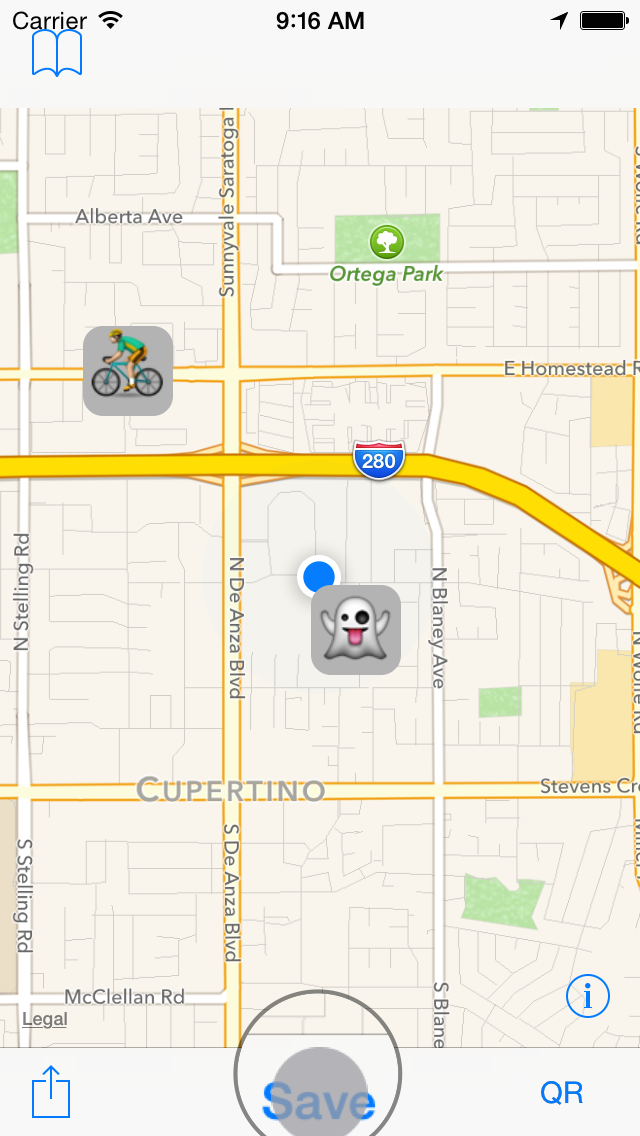
\includegraphics[width=0.7\textwidth]{../images/1_tap_to_save_place.png}


\end{center}








\end{document}